\documentclass[11pt]{article}
\usepackage[margin=0.82in]{geometry}
\usepackage{amsmath,amssymb,amsthm,graphicx,microtype}
\usepackage[T1]{fontenc}
\usepackage{lmodern}
\usepackage{enumitem}
\setlist{nosep,leftmargin=1.6em}
\newtheorem{theorem}{Theorem}
\newtheorem{corollary}{Corollary}
\newcommand{\Qp}{\mathbb Q_p}
\newcommand{\abs}[1]{\lvert#1\rvert}
\title{Why the Proposed $p$-adic Deutsch Principle Degenerates\\
\large Sharp entropy bounds and the optimal Buzano substitute}
\author{Automatic math-discovery run \texttt{fa\_banach\_001}}
\date{August 11, 2026}

\begin{document}
\maketitle

\section*{Source questions}
K.~Mahesh Krishna, \emph{$p$-adic Ghobber--Jaming Uncertainty Principle},
arXiv:2506.18913, Questions 3.7 and 3.9, asks for $p$-adic versions of the
Deutsch entropy principle and the Buzano inequality.  The source definitions
and both questions are reproduced from PDF page 10 below.

\begin{center}
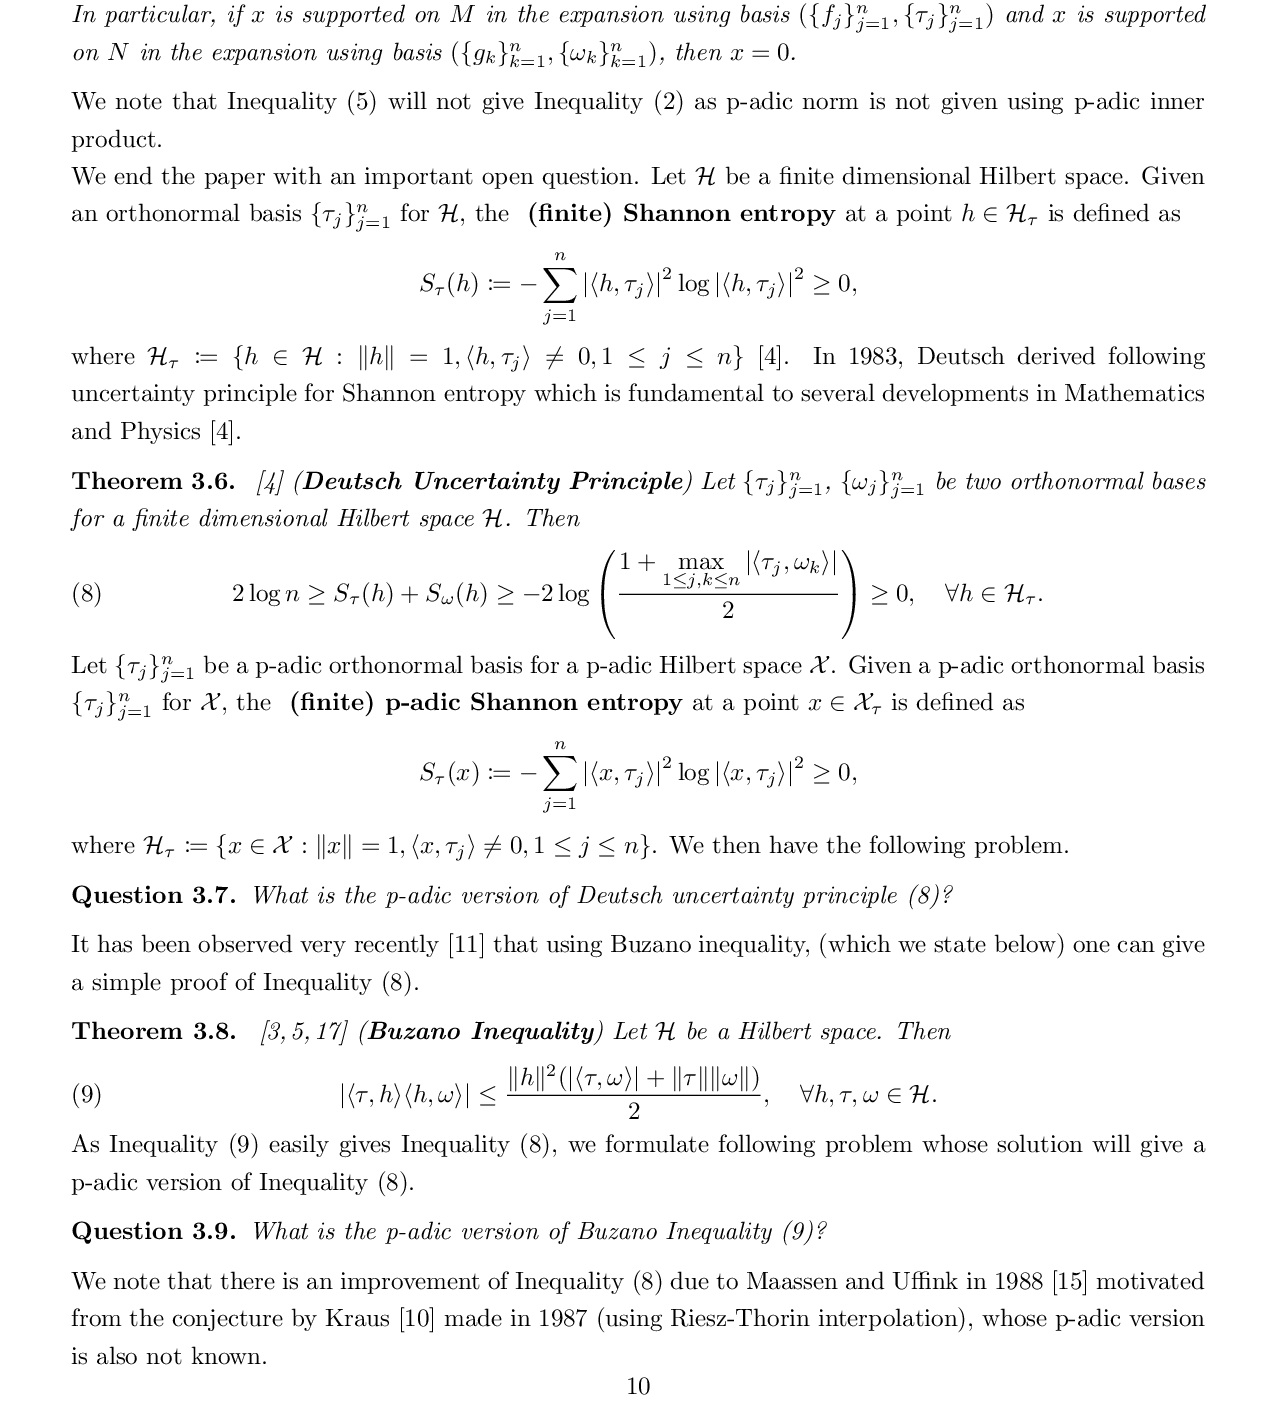
\includegraphics[width=0.88\textwidth,height=0.41\textheight,keepaspectratio]{figures/open_questions_page.jpg}
\end{center}

\section*{Resolution in one sentence}
With the definitions in the source, the coherence of two $p$-adic
orthonormal bases is \emph{always one}; the Deutsch lower bound therefore
collapses to zero, its classical upper bound is false, and the optimal
universal Buzano estimate is merely the product of two Cauchy--Schwarz
estimates.  The exact replacement bounds are given next.

\section*{Definitions}
Let $K$ be a non-Archimedean valued field and let $X$ be an $n$-dimensional
$p$-adic Hilbert space in the sense of the source.  For an orthonormal basis
$\tau=(\tau_j)_{j=1}^n$ and $\|x\|=1$, put
\[
 S_\tau(x)=-\sum_{j=1}^n \abs{\langle x,\tau_j\rangle}^2
       \log \abs{\langle x,\tau_j\rangle}^2,
\]
with $0\log0=0$.  Define $\psi(r)=-r^2\log r^2$ and
\[
 C_K=\sup\{\psi(r):r\in\abs{K^\times},\ 0<r<1\},
\]
where the supremum of the empty set is zero.

\begin{theorem}[Sharp structural answer]\label{thm:main}
Let $\tau$ and $\omega$ be orthonormal bases of $X$.
\begin{enumerate}[label=\textup{(\roman*)}]
\item Their coherence satisfies
\[
 \max_{1\le j,k\le n}\abs{\langle\tau_j,\omega_k\rangle}=1.
\]
\item For every unit vector for which the entropies are defined,
\[
 0\le S_\tau(x)+S_\omega(x)\le 2(n-1)C_K\le \frac{2(n-1)}e.
\]
For $K=\Qp$, this becomes the exact universal estimate
\[
 0\le S_\tau(x)+S_\omega(x)
 \le \frac{4(n-1)\log p}{p^2}. \tag{1}
\]
Both endpoints in (1) are attained, even with $\tau=\omega$.
\item The optimal universal Buzano substitute is
\[
 \abs{\langle u,h\rangle\langle h,v\rangle}
 \le \|u\|\,\|h\|^2\,\|v\|. \tag{2}
\]
Its constant one remains sharp under the extra condition
$\langle u,v\rangle=0$.
\end{enumerate}
\end{theorem}

\begin{proof}
The norm Parseval formula stated in the source says
\[
 \|y\|=\max_j\abs{\langle y,\tau_j\rangle}.
\]
Every $\omega_k$ has norm one.  Hence, for each fixed $k$,
$\max_j\abs{\langle\omega_k,\tau_j\rangle}=1$, proving (i).

Write $a_j=\langle x,\tau_j\rangle$.  Since $\|x\|=1$, Parseval gives
$\max_j\abs{a_j}=1$.  Thus all coordinate moduli are at most one and at
least one is one; the corresponding entropy term is zero.  Consequently
\[
 0\le S_\tau(x)\le(n-1)C_K,
\]
and the same argument for $\omega$ proves the first inequality in (ii).
The elementary real-variable maximum $\sup_{0<r\le1}\psi(r)=1/e$ proves
the field-independent bound.

For $K=\Qp$, every nonzero $r\le1$ in the value group is $r=p^{-m}$ for
an integer $m\ge0$.  When $m\ge1$,
\[
 \psi(p^{-m})=2m p^{-2m}\log p.
\]
The ratio of its value at $m+1$ to its value at $m$ is
$((m+1)/m)p^{-2}<1$.  Therefore $C_{\Qp}=2p^{-2}\log p$, which gives
(1).  In standard $\Qp^n$, take both bases canonical.  The unit vectors
\[
 x=(1,p,\ldots,p)\quad\hbox{and}\quad x=(1,1,\ldots,1)
\]
attain respectively the upper and lower endpoints; all their coordinates
are nonzero, as required by the source's domain.

Finally, the defining Cauchy--Schwarz axiom gives
\[
 \abs{\langle u,h\rangle}\le\|u\|\|h\|,
 \qquad
 \abs{\langle h,v\rangle}\le\|h\|\|v\|,
\]
and multiplication yields (2).  In standard $K^2$, set
$u=e_1$, $v=e_2$, and $h=e_1+e_2$.  Then $\langle u,v\rangle=0$, while
both sides of (2) equal one.  No universal factor smaller than one---even
at zero overlap---is possible.
\end{proof}

\section*{Consequences for the two questions}
Part (i) makes Deutsch's proposed overlap expression
\[
 -2\log\!\left(\frac{1+\max_{j,k}
 \abs{\langle\tau_j,\omega_k\rangle}}2\right)
\]
identically zero.  This is sharp as a universal lower bound by the all-unit
example above.  The classical upper bound $2\log n$ also does not survive:
over $\mathbb Q_2^8$, with equal canonical bases and
$x=(1,2,\ldots,2)$,
\[
 S_\tau(x)+S_\omega(x)=7\log2>6\log2=2\log8. \tag{3}
\]
Thus (1), not the classical interval, is the sharp answer for the entropy
defined in Question 3.7.

For Question 3.9, (2) is optimal.  The orthogonal equality example shows
precisely why a Buzano improvement depending on
$\abs{\langle u,v\rangle}$ cannot exist in this category.  It therefore
cannot supply a nonzero entropic uncertainty term.

\section*{Audit and scope}
The accompanying exact-arithmetic script verifies the discrete entropy
optimization, (3), and the orthogonal equality example.  A bounded search of
the run indexes, exact question wordings, arXiv, and the author's adjacent
$p$-adic uncertainty papers found no later answer.  Novelty confidence is
moderate pending specialist review.  The conclusion concerns exactly the
entropy and orthonormal-basis definitions printed in the source; alternative
probability normalizations may lead to different theories.

\end{document}
